% Shared style for all Git & GitHub lectures (same look as the N-body course)
\documentclass[11pt,a4paper]{article}
\usepackage[margin=2.3cm]{geometry}
\usepackage[T1]{fontenc}
\usepackage{lmodern}
\usepackage{upquote}   % straight quotes in monospaced text, so commands can be copied
\usepackage{microtype}
% keep '--' as two real hyphens in monospace text (commands like --version)
\DisableLigatures[-,<,>]{family=tt*}
\usepackage{booktabs,enumitem,graphicx,xcolor}
\usepackage{array}
\usepackage{needspace}
\usepackage{longtable}
\usepackage{float}
\usepackage{tikz}
\usetikzlibrary{arrows.meta,calc,positioning,decorations.pathreplacing,shapes.geometric,fit,backgrounds}
\usepackage[most]{tcolorbox}
\usepackage{listings}
\usepackage{fancyhdr}
\usepackage[colorlinks=true,linkcolor=blue!50!black,urlcolor=blue!50!black,citecolor=blue!50!black]{hyperref}

\setlength{\parindent}{0pt}
\setlength{\parskip}{0.6em}
\setlength{\abovecaptionskip}{4pt}
\usepackage[font=small,labelfont=bf]{caption}
\setlist{itemsep=0.2em,topsep=0.3em}

% ---------- colours ----------
\definecolor{cbg}{HTML}{F6F8FA}
\definecolor{ckw}{HTML}{0B5CAD}
\definecolor{ccm}{HTML}{6A737D}
\definecolor{cst}{HTML}{B5451B}
\definecolor{cpart}{HTML}{1F6FB2}
\definecolor{cheavy}{HTML}{C0392B}
\definecolor{cgreen}{HTML}{2E8B57}

% ---------- terminal listings ----------
% In a terminal session, lines starting with "$" are what YOU type.
% Everything else is what Git prints back.
\lstdefinestyle{term}{
  basicstyle=\ttfamily\small, backgroundcolor=\color{cbg},
  frame=single, rulecolor=\color{black!15}, showstringspaces=false,
  breaklines=true, columns=fullflexible, keepspaces=true,
  aboveskip=0.6em, belowskip=0.6em, xleftmargin=4pt, xrightmargin=4pt,
  literate={\$\ }{{\textcolor{cgreen}{\$\ }}}2,
  upquote=true
}
\lstset{style=term}
\newcommand{\code}[1]{\texttt{\small #1}}

% ---------- boxes ----------
\newtcolorbox{history}{colback=yellow!8,colframe=orange!60!black,
  title={History},fonttitle=\bfseries\small,left=4pt,right=4pt,top=2pt,bottom=2pt}
\newtcolorbox{quickfact}{colback=purple!4,colframe=purple!55!black,
  title={Quick fact},fonttitle=\bfseries\small,left=4pt,right=4pt,top=2pt,bottom=2pt}
\newtcolorbox{keyidea}{colback=blue!4,colframe=blue!50!black,
  title={Key idea},fonttitle=\bfseries\small,left=4pt,right=4pt,top=2pt,bottom=2pt}
\newtcolorbox{pitfall}{colback=red!4,colframe=red!55!black,
  title={Pitfall},fonttitle=\bfseries\small,left=4pt,right=4pt,top=2pt,bottom=2pt}
\newtcolorbox{tryit}{colback=teal!5,colframe=teal!55!black,
  title={Try it},fonttitle=\bfseries\small,left=4pt,right=4pt,top=2pt,bottom=2pt,breakable}
\newtcolorbox{homework}[1]{colback=green!4,colframe=green!40!black,
  title={Homework #1},fonttitle=\bfseries\small,left=4pt,right=4pt,top=2pt,bottom=2pt,
  breakable}
\newtcolorbox{goals}{colback=gray!6,colframe=gray!60!black,
  title={Learning goals},fonttitle=\bfseries\small,left=4pt,right=4pt,top=2pt,bottom=2pt}

% Solutions always start on a fresh page, behind a clear warning.
\newcommand{\solutionspage}{%
  \clearpage
  \begin{tcolorbox}[colback=red!6,colframe=red!60!black,halign=center]
    {\Large\bfseries Solutions}\\[0.3em]
    {\small Stop here if you have not tried the homework yet.\\
    Attempt every task first, run the checker, and only then read on.}
  \end{tcolorbox}
}

% ---------- Git diagram styles (TikZ) ----------
\tikzset{
  commit/.style={circle,draw=black!70,fill=blue!10,minimum size=7mm,inner sep=0pt,font=\scriptsize\ttfamily},
  newcommit/.style={commit,fill=orange!25,dashed},
  tag/.style={draw,rounded corners=2pt,font=\scriptsize\ttfamily,inner sep=2pt},
  branchtag/.style={tag,fill=green!15,draw=green!40!black},
  headtag/.style={tag,fill=yellow!30,draw=orange!70!black},
  remotetag/.style={tag,fill=purple!10,draw=purple!60!black},
  area/.style={draw,rounded corners,minimum height=11mm,minimum width=33mm,align=center,font=\small},
  cmdarrow/.style={->,thick,>=Stealth},
  link/.style={->,thick,>=Stealth,black!70},
}

% ---------- header ----------
\pagestyle{fancy}
\fancyhf{}
\renewcommand{\headrulewidth}{0.3pt}
\fancyfoot[C]{\thepage}
\newcommand{\lecturetitle}[3]{%
  \fancyhead[L]{\small\textit{Git \& GitHub from Zero}}
  \fancyhead[R]{\small Lecture #1}
  \begin{center}
    {\Large\bfseries Lecture #1}\\[0.4em]
    {\LARGE\bfseries #2}\\[0.4em]
    {\small #3}
  \end{center}
  \vspace{0.5em}
}

\begin{document}
\lecturetitle{1}{First Steps: The Terminal, Configuration, and Your First Repository}{Moving around in a terminal, telling Git who you are, \code{git init}, and \code{git status}}

\begin{goals}
\begin{itemize}
  \item Move around the file system and create files from a terminal.
  \item Tell Git who you are, and understand the three places where settings live.
  \item Turn an ordinary folder into a Git repository with \code{git init}.
  \item Explain what the hidden \code{.git} folder is, and why you must not delete it.
  \item Read the output of \code{git status}.
  \item Find help for any Git command on your own.
\end{itemize}
\end{goals}

\section{The terminal in ten minutes}

Git is used mostly through a \textbf{terminal}: a window where you type a command, press Enter, and the computer replies with text. Point-and-click programs for Git exist, but the terminal is the same on every computer, it is what every tutorial and every colleague uses, and it shows you exactly what Git is doing. A little practice here pays off in every later lecture.

The program inside the terminal that reads your commands is called a \textbf{shell}. With Git Bash on Windows, and on Linux, it is usually \code{bash}; on macOS it is \code{zsh}. (Windows also has PowerShell, which differs: use Git Bash in this course.) The commands in this lecture work the same in all of them.

\begin{history}
The Unix shell dates from 1971. Bash (``Bourne-again shell'') was first released in 1989 as part of the GNU project and became the default on most Linux systems. Git was designed on Linux, which is why its commands feel like shell commands.
\end{history}

\subsection{The prompt and your location}

When the terminal is ready for a command it shows a \textbf{prompt}. It usually ends with \code{\$} or \code{\%}. Its exact look differs between computers, so in this course we write just \code{\$}. You do \emph{not} type the \code{\$}.

At every moment the terminal is ``standing'' in one folder, called the \textbf{current directory} or \textbf{working directory}. Almost every command acts on the folder you are standing in, so always know where you are.

\begin{lstlisting}
$ pwd
/Users/sam
$ ls
Desktop    Documents    Downloads
\end{lstlisting}

\code{pwd} (``print working directory'') prints where you are. \code{ls} (``list'') shows what is inside. Your output will differ.

\subsection{Moving around}

Folders form a tree: every folder sits inside another folder, up to the top (the \emph{root}).

\begin{figure}[H]
\centering
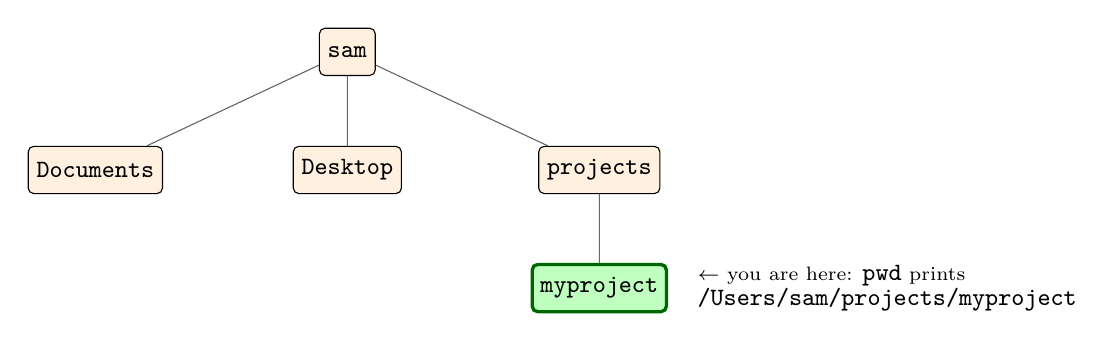
\begin{tikzpicture}[
  fold/.style={draw,rounded corners=2pt,fill=orange!12,font=\small\ttfamily,minimum height=6mm,inner sep=3pt},
  here/.style={fold,fill=green!25,very thick,draw=green!40!black},
  lvl/.style={sibling distance=3cm},
  edge from parent/.style={draw,black!60}]
  \node[fold] {sam}
    child[sibling distance=3.2cm] { node[fold] {Documents} }
    child[sibling distance=3.2cm] { node[fold] {Desktop} }
    child[sibling distance=3.2cm] { node[fold] {projects}
       child { node[here] (mp) {myproject} } };
  \node[font=\scriptsize,anchor=west,align=left] at ($(mp.east)+(0.25,0)$) {$\leftarrow$ you are here: \code{pwd} prints\\\code{/Users/sam/projects/myproject}};
\end{tikzpicture}
\caption{A folder tree (a home folder named \code{sam}). The green folder is the current directory.}
\label{fig:tree}
\end{figure}

\begin{center}
\small
\begin{tabular}{@{}l >{\raggedright\arraybackslash}p{9cm}@{}}
\toprule
Command & What it does \\
\midrule
\code{pwd} & Print the current directory. \\
\code{ls} & List what is in the current directory. \code{ls -a} also shows \emph{hidden} files (names starting with a dot). \\
\code{cd projects} & Change directory: go into the folder \code{projects}. \\
\code{cd ..} & Go up one level (\code{..} means ``the parent folder''). \\
\code{cd} or \code{cd \~{}} & Go back to your home folder (\code{\~{}} is shorthand for it). \\
\code{mkdir name} & Make a new folder. \\
\code{echo "text" > file} & Write the text into a file. The symbol \code{>} sends a command's output into a file instead of the screen, creating the file or \emph{replacing} it; \code{>>} \emph{appends} instead. \\
\code{cat file} & Print the contents of a file. \\
\code{rm file} & Delete a file \emph{permanently} (there is no recycle bin). \code{rm -r folder} deletes a folder and everything in it. Use with care. \\
\bottomrule
\end{tabular}
\end{center}

\begin{lstlisting}
$ cd projects            # go into projects
$ mkdir myproject        # make a new folder
$ cd myproject           # go into it
$ pwd
/Users/sam/projects/myproject
$ echo "Hello Git" > hello.txt
$ ls
hello.txt
$ cat hello.txt
Hello Git
$ cd ..                  # back up to projects
\end{lstlisting}

\begin{keyidea}
Press the \textbf{Tab} key to auto-complete file and folder names, and the \textbf{Up arrow} to bring back your previous command. Both save a lot of typing and a lot of typos.
\end{keyidea}

\begin{pitfall}
Spaces separate the parts of a command, so a folder name with a space must be put in quotes (\code{cd "my project"}). To avoid this, use names without spaces, such as \code{my-project}. Also type names exactly: Linux is case sensitive (\code{Hello.txt} and \code{hello.txt} are different files), while macOS and Windows usually ignore case but keep it.
\end{pitfall}

\begin{tryit}
Open your terminal and, without looking above, do this: print where you are, list the files, go into your \code{Documents} folder, make a folder called \code{terminal-play}, go into it, create a file \code{a.txt} containing the word \code{hi}, print the file, go back up one level, and finally clean up with \code{rm -r terminal-play}.
\end{tryit}

\section{Telling Git who you are}

Every saved version in Git records \emph{who} made it. Git does not guess: you must give it your name and email once. This is the step you already did in Homework 0. Here we see what it really did.

\begin{lstlisting}
$ git config --global user.name "Your Name"
$ git config --global user.email "you@example.com"
\end{lstlisting}

The pattern is \code{git config <scope> <setting> <value>}. Settings have a dotted name such as \code{user.name}. The word \code{--global} says \emph{where} to store the setting. There are three places, called \textbf{scopes}:

\begin{figure}[H]
\centering
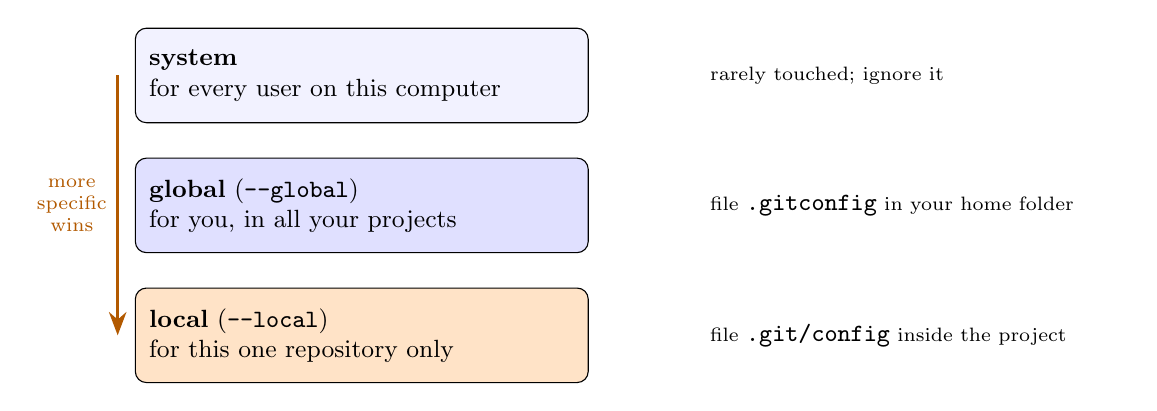
\begin{tikzpicture}[
  lev/.style={draw,rounded corners,align=left,font=\small,minimum height=12mm,text width=5.4cm,inner sep=5pt},
  weak/.style={lev,fill=blue!5}, mid/.style={lev,fill=blue!12}, strong/.style={lev,fill=orange!22}]
  \node[weak]   (s) at (0,3.3) {\textbf{system}\\for every user on this computer};
  \node[mid]    (g) at (0,1.65) {\textbf{global} (\code{--global})\\for you, in all your projects};
  \node[strong] (l) at (0,0)   {\textbf{local} (\code{--local})\\for this one repository only};
  \node[font=\scriptsize,anchor=west,text width=5.2cm,align=left] at (4.3,3.3) {rarely touched; ignore it};
  \node[font=\scriptsize,anchor=west,text width=5.2cm,align=left] at (4.3,1.65) {file \code{.gitconfig} in your home folder};
  \node[font=\scriptsize,anchor=west,text width=5.2cm,align=left] at (4.3,0) {file \code{.git/config} inside the project};
  \draw[->,very thick,>=Stealth,orange!70!black] (-3.1,3.3) -- node[left,font=\scriptsize,align=center] {more\\specific\\wins} (-3.1,0);
\end{tikzpicture}
\caption{Where settings live. If the same setting appears in several places, the most specific one wins.}
\label{fig:scopes}
\end{figure}

The usual use of this: your global email is your personal one, but for one particular project (say, for work) you want a different email. Setting it \emph{inside that repository} overrides the global value only there.

To see all your settings, or just one, and \emph{where} each comes from:

\begin{lstlisting}
$ git config --list --show-origin
file:/home/sam/.gitconfig       user.name=Your Name
file:/home/sam/.gitconfig       user.email=you@example.com
file:/home/sam/.gitconfig       init.defaultbranch=main
$ git config user.name
Your Name
\end{lstlisting}
(Your list will have more lines. Git also lowercases setting names when it lists them.) The \code{init.defaultbranch} line is the setting from Homework 0.3: the name given to the first branch of every new repository.

\Needspace{9\baselineskip}
Inside a repository, \code{git config} with no scope sets the \emph{local} value, which then wins over the global one:
\begin{lstlisting}
$ git config user.email "work@example.com"    # local (inside a repository)
$ git config user.email                       # the winner is shown
work@example.com
$ git config --global user.email              # global value is untouched
you@example.com
\end{lstlisting}


\begin{pitfall}
The email in your Git settings is written into every version you save, and becomes public if you push to a public repository. If you do not want your real address public, GitHub offers a private ``noreply'' address in its settings. We return to this in Lecture 6.
\end{pitfall}

\section{Creating a repository}

A \textbf{repository} (or \emph{repo}) is a project folder that Git is keeping track of. Turning an ordinary folder into a repository takes one command, run from inside the folder:

\begin{lstlisting}
$ cd ~/projects/myproject
$ git init
Initialized empty Git repository in /Users/sam/projects/myproject/.git/
$ ls
hello.txt
$ ls -a
.    ..    .git    hello.txt
\end{lstlisting}

Nothing visible changed in your files, but a new hidden folder, \code{.git}, has appeared. (Output of \code{ls -a} also lists \code{.} and \code{..}: these mean ``this folder'' and ``the parent folder''.)

\begin{figure}[H]
\centering
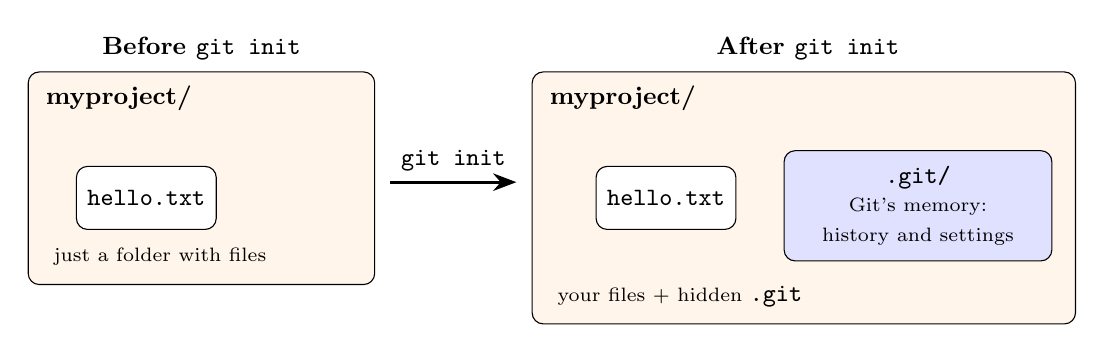
\begin{tikzpicture}[
  box/.style={draw,rounded corners,minimum height=8mm,font=\small\ttfamily,inner sep=4pt}]
  \node[font=\small\bfseries] at (-3.2,3.0) {Before \code{git init}};
  \draw[rounded corners,fill=orange!8] (-5.4,0) rectangle (-1.0,2.7);
  \node[font=\small\bfseries,anchor=north west] at (-5.3,2.65) {myproject/};
  \node[box,fill=white] at (-3.9,1.1) {hello.txt};
  \node[font=\scriptsize,anchor=west] at (-5.2,0.35) {just a folder with files};

  \draw[->,very thick,>=Stealth] (-0.8,1.3) -- node[above,font=\small\ttfamily] {git init} (0.8,1.3);

  \node[font=\small\bfseries] at (4.5,3.0) {After \code{git init}};
  \draw[rounded corners,fill=orange!8] (1.0,-0.5) rectangle (7.9,2.7);
  \node[font=\small\bfseries,anchor=north west] at (1.1,2.65) {myproject/};
  \node[box,fill=white] at (2.7,1.1) {hello.txt};
  \node[box,fill=blue!12,minimum width=3.4cm,minimum height=14mm,align=center] (g) at (5.9,1.0) {.git/\\[-1pt]\scriptsize\rmfamily Git's memory:\\\scriptsize\rmfamily history and settings};
  \node[font=\scriptsize,anchor=west] at (1.2,-0.15) {your files + hidden \code{.git}};
\end{tikzpicture}
\caption{A repository is a normal folder plus a hidden \code{.git} folder. Your own files are untouched.}
\label{fig:init}
\end{figure}

\begin{keyidea}
A repository is \emph{not} a special kind of file or a database somewhere else. It is a folder that contains a \code{.git} subfolder. The \code{.git} folder holds the whole history of the project and the repository's own settings. Delete \code{.git} and the folder is an ordinary folder again, with its history gone.
\end{keyidea}

You can look inside, but do not edit it by hand:

\begin{lstlisting}
$ ls .git
HEAD    config    description    hooks    info    objects    refs
$ cat .git/HEAD
ref: refs/heads/main
\end{lstlisting}
(You may see a few more entries; it depends on your Git.) You do not need to understand these yet. Lecture 10 opens this folder properly. For now notice two things: \code{config} is the file for the \emph{local} settings of Figure~\ref{fig:scopes}, and \code{HEAD} says which branch you are on (here \code{main}, the name you set in Homework 0).

\begin{quickfact}
If your new repository does not start on \code{main} (for example you skipped Homework 0.3), create it with \code{git init -b main}, or rename the branch afterwards with \code{git branch -m main}. Check the current branch name any time with \code{git status}.
\end{quickfact}

\begin{pitfall}
\textbf{Run \code{git init} once per project, and only inside the project folder.} Never run it in your home folder or your Desktop: Git would try to track everything there. Also do not create a repository inside another repository; the inner one confuses the outer one. If you are unsure where you are, run \code{pwd} first. (In this course, your practice repositories live in the \code{practice/} folder of the course folder, which is itself a repository. That is why you must \code{git init} inside each practice folder, so that it becomes its own, separate repository.)
\end{pitfall}

\section{Asking Git what is going on: \texttt{git status}}

The command you will type most often is \code{git status}. It tells you which branch you are on and what changed since the last saved version. Try it in your new repository, first with only the file \code{hello.txt} from before:

\begin{lstlisting}
$ git status
On branch main

No commits yet

Untracked files:
  (use "git add <file>..." to include in what will be committed)
	hello.txt

nothing added to commit but untracked files present (use "git add" to track)
\end{lstlisting}

Read it line by line:
\begin{description}[leftmargin=1.2em,style=nextline]
\item[\code{On branch main}] You are on the branch called \code{main}. (Branches are Lecture 4.)
\item[\code{No commits yet}] You have not saved any version. A \emph{commit} is one saved version of the project. You make the first one in Lecture 2.
\item[\code{Untracked files}] Git can see \code{hello.txt} in the folder, but it is not tracking it: it is not part of any saved version. The line in brackets tells you the command to use next, \code{git add}. Git's messages often tell you the next step, so read them.
\end{description}

In an empty repository the message ends with \code{nothing to commit (create/copy files and use "git add" to track)}.

\begin{tryit}
Create a new folder, run \code{git init} in it, and run \code{git status}. Now add a file with \code{echo "x" > a.txt} and run \code{git status} again. What changed in the output? Then create a second file and look again.
\end{tryit}

\begin{keyidea}
\code{git status} never changes your files or your history. It is always safe, so run it whenever you are unsure. A common habit: run it before and after every other Git command.
\end{keyidea}

\section{Getting help}

No one remembers all of Git. Two ways to look things up from the terminal:

\begin{lstlisting}
$ git config -h          # short summary of options
$ git help config        # full manual page (same as: git config --help)
\end{lstlisting}
The full manual opens in a viewer: press the arrow keys or space to scroll and \code{q} to quit. On Windows it opens in your web browser. The same manuals are online at \url{https://git-scm.com/docs}.

Error messages are also help: read them from the top. Git usually says what is wrong and often what to do.

\textbf{Your workflow so far:} open a terminal, \code{cd} to the project, \code{git init} (once only), create or edit files, \code{git status}, and repeat. In Lecture 2 a ``save a version'' step joins the loop.


\Needspace{42\baselineskip}
\section{Homework 1}

\begin{homework}{1: Your first repository}
All work happens inside the \code{practice/} folder of the course folder. From the course folder (\code{LearningGit/}), run:
\begin{lstlisting}
$ bash codeHints/L01/setup_hw1.sh
\end{lstlisting}
It only prepares the \code{practice/} folder and prints a reminder. \textbf{You do the tasks yourself}; the setup script does not build the repository for you.

\begin{description}[leftmargin=1.2em,style=nextline]
\item[1.1 Folder] Create a folder \code{hw1} inside \code{practice/} and go into it.
\item[1.2 Repository] Turn \code{hw1} into a Git repository whose first branch is called \code{main}. (\emph{Warning:} \code{practice/} sits inside the course repository. If \code{git status} mentions paths such as \code{practice/hw1/}, you forgot \code{git init} in \code{hw1}.)
\item[1.3 A file] Create a file \code{hello.txt} containing the single line \code{Hello Git}.
\item[1.4 Local identity] Set a \emph{local} identity inside this repository only: name \code{Practice User} and email \code{practice@example.com}. Your global settings must stay as they were.
\item[1.5 Status] Save the output of \code{git status} into a file called \code{status.txt} (hint: \code{git status > status.txt}).
\item[1.6 Question] Create a file \code{answer.txt} whose only content is the name of the hidden folder (its name starts with a dot) in which Git keeps a project's history.
\end{description}

\textbf{Check yourself:} from the course folder run \code{bash codeHints/L01/check\_hw1.sh}. Aim for all \code{PASS}, then compare with the solutions at the end of this lecture (or in \code{solutions/L01/}). Do not commit anything yet: you learn how in Lecture 2.
\end{homework}

\section{Summary}

\begin{itemize}
  \item The terminal runs commands in a current directory: \code{pwd}, \code{ls}, \code{cd}, \code{mkdir}, \code{echo}, \code{cat}.
  \item \code{git config} stores settings at three scopes (system, global, local); the most specific wins.
  \item \code{git init} makes a folder a repository by creating a hidden \code{.git} folder that holds the history.
  \item \code{git status} is safe and read-only: run it often and read its messages. \code{git help <command>} shows the manual.
\end{itemize}

\textbf{Further reading:} \emph{Pro Git} (\url{https://git-scm.com/book}), Chapters 1.6 and 2.1; manual pages \code{git help init}, \code{config}, \code{status}.

\solutionspage

\section*{Solutions to Homework 1}

Run these from the course folder \code{LearningGit/}. Your prompt and the exact path will differ.

\begin{lstlisting}
$ cd practice
$ mkdir hw1
$ cd hw1
$ git init -b main
Initialized empty Git repository in .../practice/hw1/.git/
$ echo "Hello Git" > hello.txt
$ git config --local user.name "Practice User"
$ git config --local user.email "practice@example.com"
$ git status > status.txt
$ echo ".git" > answer.txt
\end{lstlisting}

\textbf{1.1.} \code{mkdir hw1} creates the folder and \code{cd hw1} enters it (do this from inside \code{practice/}).

\textbf{1.2.} \code{git init} creates the repository. The branch name comes from the global setting you made in Homework 0; \code{git init -b main} states it explicitly (Git 2.28 or newer), so it is the safe choice. If you forgot and your branch has another name (for example \code{master}), rename it with \code{git branch -m main}.

\textbf{1.3.} \code{echo "Hello Git" > hello.txt} writes one line. Check with \code{cat hello.txt}. Note that \code{>} \emph{replaces} the file each time; \code{>>} would append.

\textbf{1.4.} \code{--local} is the default for \code{git config} inside a repository, so you could omit it, but writing it makes the intent clear. Verify where the values come from, and that your global ones are unchanged:
\begin{lstlisting}
$ git config --show-origin user.name
file:.git/config        Practice User
$ git config --global user.name
Your Name
\end{lstlisting}

\textbf{1.5.} After the redirect, \code{status.txt} should look like this (it lists itself as untracked too, because the file already exists when Git runs):
\begin{lstlisting}
On branch main

No commits yet

Untracked files:
  (use "git add <file>..." to include in what will be committed)
	hello.txt
	status.txt

nothing added to commit but untracked files present (use "git add" to track)
\end{lstlisting}

\textbf{1.6.} The folder is \code{.git}. The file may contain \code{.git} or \code{.git/}.

\Needspace{8\baselineskip}
\textbf{Common mistakes.}
\begin{itemize}
  \item Running \code{git init} in the wrong folder (check with \code{pwd}). Do \emph{not} delete anything until you are sure: \code{rm -r .git} is only safe in a folder you created for this exercise and just ran \code{git init} in by mistake. Never run it inside \code{LearningGit/} itself, because that would erase the course repository's history.
  \item Forgetting that \code{git init} is needed inside \code{practice/hw1}. Without it, \code{git status} would talk about the \emph{course} repository above it.
  \item Typing the \code{\$} at the start of a command.
  \item Using \code{--global} instead of \code{--local} in 1.4. That changes your name for every project. Undo it by setting your real name and email again with \code{git config --global}.
\end{itemize}


\end{document}
